\date{}
\documentclass[12pt]{article}
\usepackage{mathptmx}% http://ctan.org/pkg/mathptmx
\usepackage[top=1.5cm, bottom=2.2cm, left=3cm, right=2cm, headsep=1.2cm, footskip=1cm, headheight=0.3cm, textheight=24.5cm, textwidth=16cm]{geometry}
\usepackage{fancyhdr}
\usepackage{graphicx}
\graphicspath{ {images/} }
\makeatletter
\def\@seccntformat#1{%
  \expandafter\ifx\csname c@#1\endcsname\c@section\else
  \csname the#1\endcsname\quad
  \fi}
\makeatother
\renewcommand{\baselinestretch}{1.5}
\title{\textbf{Chapter 3}\vspace{-6ex}}


\begin{document}
\maketitle

\pagenumbering{arabic}
\setcounter{page}{8}

\begin{center}
\section{System Analysis}
\end{center}

\setcounter{section}{3}
\subsection{Functional Requirements}
Functional requirements describe all the required functionality or system services. Functionality is described as a set of inputs, the behaviour, and outputs expected from the system. They are functions or features that must be included in a system in order to satisfy the business needs and must be acceptable to the system users.\newline
The proposed system should provide following functional requirements:
\begin{itemize}
    \item The system requires the chrome extension to automatically take the URL from the web browser when the web page is loaded.
    \item The chrome extension must be able to pass the URL to the cloud where the model is stored.
    \item The cloud must be able to successfully extract the features of URL and feed to the model.
    \item The model must be able to predict to the URL as phished or safe to the best possible accuracy of the algorithm used.
    \item The Cloud must be able to give the result back to chrome extension.
    \item The chrome extension must alert the user regarding the same.
\end{itemize}

\subsection{Non-Functional Requirements}
The non-functional requirements define the properties and constraints of the system. Non-functional requirements impose constraints on the design or implementation. It is used to judge the operation of a system.

\newgeometry{top=3cm, bottom=2.2cm, left=3cm, right=2cm, headsep=1.2cm, footskip=1cm, headheight=0.3cm, textheight=24.5cm, textwidth=16cm}

\pagestyle{fancy}
\fancyhf{}
\renewcommand{\headrulewidth}{0pt}
\lhead{Chapter 3}
\rhead{System Analysis}
\cfoot{\thepage}

The proposed system should provide following non-functional requirements:\newline
\begin{itemize}
    \item Acceptable – Verified as meeting the stated objectives
    \item Accessible – Accessible from different devices
    \item Availability – 24 x 7 x 365. 
    \item Secured and Restorable – System and data backups. Business Continuity / Disaster
    \item Maintainability- The ease with which the system can be changed, whether for bug fixes or to add new functionality.
    \item Modifiable and Extensible – Ease and cost to make ongoing changes
    \item Responsive / Performance – Response times. Speed of page loads and calculations
    \item Reliable – Consistent and dependable quality of service
    \item Usable – Easy to use by target users. Both humans and web crawlers
\end{itemize}

\subsection{Specific Requirements}
\subsubsection*{Hardware Requirements}
\begin{itemize}
    \item Hard Disk: 40 GB hard disk space and above.
    \item RAM: Minimum 512 MB and above.
    \item 1GHZ processor
\end{itemize}
\subsubsection*{Software Requirements}
\begin{itemize}
    \item Chrome Browser.
    \item Middle-ware: Algorithmia (Cloud API provider and storage provider).
    \item Programming language for coding: JavaScript/Python. 
    \item An internet connection is required.
\end{itemize}

\newgeometry{top=3cm, bottom=2.2cm, left=3cm, right=2cm, headsep=1.2cm, footskip=1cm, headheight=0.3cm, textheight=24.5cm, textwidth=16cm}

\pagestyle{fancy}
\renewcommand{\headrulewidth}{0pt}
\lhead{3.4}
\rhead{Use Case Diagram}


\subsection{Use Case Diagram}
\begin{figure}[h]
\centering
\graphicspath{ Diagrams/ }
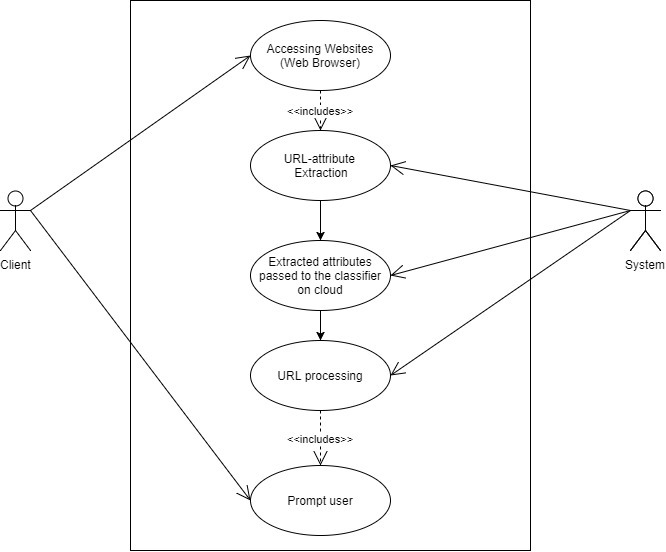
\includegraphics[scale=0.7]{Diagrams/use_case.jpg}
\setcounter{figure}{0}
\renewcommand{\thefigure}{\arabic{section}.\arabic{subsection}.\arabic{figure}}
\caption{Use Case diagram for Detecting Phishing websites using Data Mining}
\end{figure}\newline
In figure 1, we have shown the use case diagram for Detecting Phishing websites using Data Mining. The client just has to just visit the website and it is solely the job of the system to decide whether the website is safe of phished. The System here includes the Chrome extension as well as the Classifier residing on the cloud.

\newgeometry{top=3cm, bottom=2.2cm, left=3cm, right=2cm, headsep=1.2cm, footskip=1cm, headheight=0.3cm, textheight=24.5cm, textwidth=16cm}

\pagestyle{fancy}
\fancyhf{}
\renewcommand{\headrulewidth}{0pt}
\lhead{Chapter 3}
\rhead{System Analysis}
\cfoot{\thepage}

\subsubsection*{Use case Description:}
\textbf{Actors:},\textit{Client} and the \textit{System} are the two end users for Phishing Detection.

\begin{table}[h]
\caption{Use Case Description for UC01- Accessing websites (web browser).}
\centering
\begin{tabular}{|p{3cm}|p{10cm}|}
\hline
    Use Case & Accessing Websites (Web Browser)  \\
    \hline
    Use Case ID & UC01 \\
    \hline
    Actor & Client \\
    \hline
    Description & Client visits various websites through a web client i.e. Web Browser, which may be safe or Phished. \\
    \hline
\end{tabular}
\end{table}

\begin{table}[h]
\caption{Use Case Description for UC02-URL attribute extraction.}
\centering
\begin{tabular}{|p{3cm}|p{10cm}|}
\hline
    Use Case & URL-attribute extraction  \\
    \hline
    Use Case ID & UC02 \\
    \hline
    Actor & System \\
    \hline
    Description & The visited URL will be fetched by the Chrome extension and various attributes will be extracted from it. \\
    \hline
\end{tabular}
\end{table}

\begin{table}[h]
\caption{Use Case Description for UC03-attribute extraction.}
\centering
\begin{tabular}{|p{3cm}|p{10cm}|}
\hline
    Use Case & Extracted attributes passed to the classifier on cloud \\
    \hline
    Use Case ID & UC03 \\
    \hline
    Actor & System \\
    \hline
    Description & The attributes extracted by the Chrome Extension are passed onto the classifier on cloud for testing purpose. \\
    \hline
\end{tabular}
\end{table}

\newgeometry{top=3cm, bottom=2.2cm, left=3cm, right=2cm, headsep=1.2cm, footskip=1cm, headheight=0.3cm, textheight=24.5cm, textwidth=16cm}

\pagestyle{fancy}
\renewcommand{\headrulewidth}{0pt}
\lhead{3.4}
\rhead{Use Case Diagram}


\begin{table}[h]
\caption{Use Case Description for UC04-URL processing.}
\centering
\begin{tabular}{|p{3cm}|p{10cm}|}
\hline
    Use Case & URL Processing  \\
    \hline
    Use Case ID & UC04 \\
    \hline
    Actor & System \\
    \hline
    Description & Here, the testing of the URL attributes is done using appropriate classifier. \\
    \hline
\end{tabular}
\end{table}

\begin{table}[h]
\caption{Use Case Description for UC05-prompting user}
\centering
\begin{tabular}{|p{3cm}|p{10cm}|}
\hline
    Use Case & Prompt User  \\
    \hline
    Use Case ID & UC05 \\
    \hline
    Actor & Client \\
    \hline
    Description & The predicted output is given to the user whether the website is phished or safe. \\
    \hline
\end{tabular}
\end{table}


\end{document}
